

\begin{figure}
\begin{subfigure}{.5\linewidth}
\centering

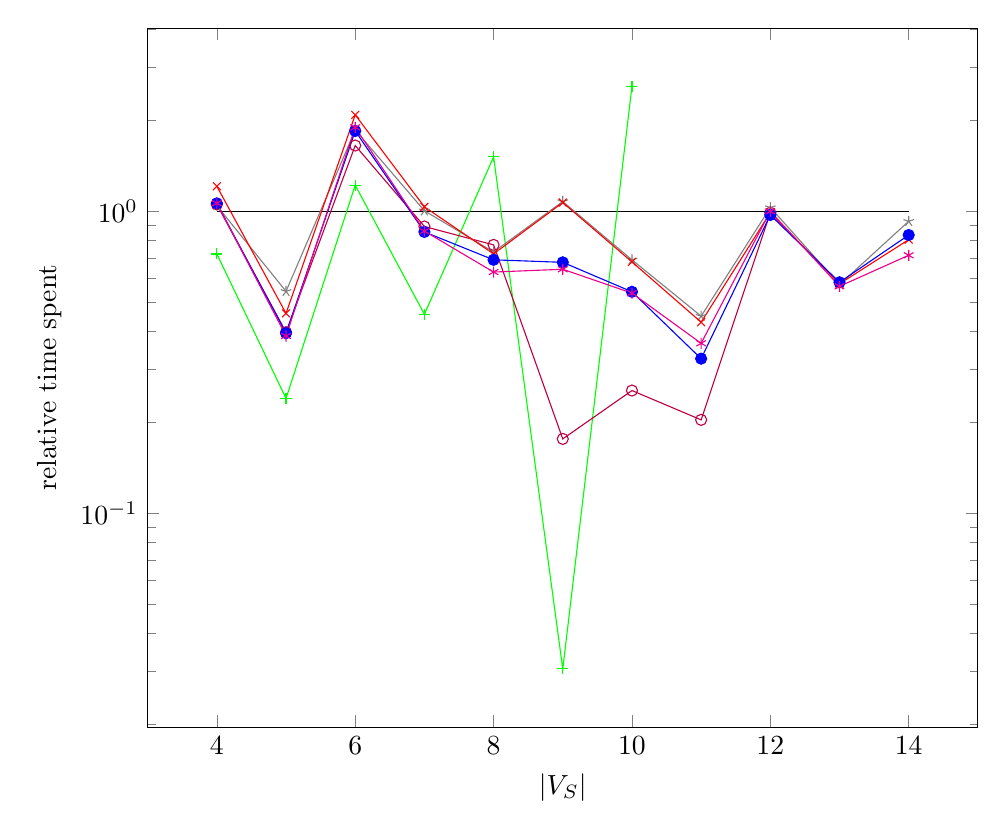
\begin{tikzpicture}
    \begin{axis}[
        xlabel=$|V_S|$,
        ylabel=relative time spent,
        ymode=log,
        legend style={at={(0.9,0.1)},anchor=south east},
        width=\textwidth,
		y tick label style={/pgf/number format/sci},
    ]


\addplot [mark=none, black] plot coordinates {
        (4,1) (14, 1)};
%\addlegendentry{No contraction}

\addplot[
        mark=+,
        green,
    ] plot coordinates {
        (4,0.7216233008103387)
        (5,0.23979959256395095)
        (6,1.219055373815801)
        (7,0.45549808099886696)
        (8,1.5129803175671477)
        (9,0.030491817239336187)
        (10,2.587109386205813)
};
%    \addlegendentry{CP}

\addplot[
        mark=o,
        purple,
    ] plot coordinates {
        (4,1.0524711376958586)
        (5,0.397430142997267)
        (6,1.649483210945216)
        (7,0.8895236575282935)
        (8,0.7731988158571639)
        (9,0.17613609063915775)
        (10,0.25469552245651866)
        (11,0.20364401173813004)
        (12,0.9888612062339083)
};
%    \addlegendentry{GDFS O IP}

\addplot[
        mark=star,
        gray,
    ] plot coordinates {
        (4,1.0424825365257937)
        (5,0.5426295402334718)
        (6,1.855682646836014)
        (7,1.0030303685825734)
        (8,0.732541042585068)
        (9,1.0760282051348324)
        (10,0.6898563436739937)
        (11,0.4490497012282625)
        (12,1.0279132116341756)
        (13,0.5714085857541255)
        (14,0.9256163980737115)
};
%    \addlegendentry{GDFS C}

\addplot[
        mark=x,
        red,
    ] plot coordinates {
        (4,1.208819655001192)
        (5,0.4586488473969574)
        (6,2.083424951258273)
        (7,1.0333509881095415)
        (8,0.7217323256161471)
        (9,1.067791165771744)
        (10,0.6792053743658721)
        (11,0.42883471023577835)
        (12,0.9888018890272706)
        (13,0.5747328589505348)
        (14,0.8046705504898993)
};
%    \addlegendentry{DFS}

\addplot[
        mark=*,
        blue,
    ] plot coordinates {
        (4,1.0612749917741098)
        (5,0.3945236842140588)
        (6,1.8429590288918432)
        (7,0.8535961630308873)
        (8,0.6899304068674341)
        (9,0.6769900545914925)
        (10,0.5407198063482145)
        (11,0.3247299866242016)
        (12,0.9713817184344807)
        (13,0.5813925975914811)
        (14,0.8336248540971392)
};
%    \addlegendentry{K-Path}

\addplot[
        mark=asterisk,
        magenta,
    ] plot coordinates {
        (4,1.0622283595408073)
        (5,0.38615187683924507)
        (6,1.894044220650229)
        (7,0.8590163375653131)
        (8,0.6286080587791637)
        (9,0.6420560054284833)
        (10,0.5352470679476732)
        (11,0.36511431500997044)
        (12,0.9985286266608072)
        (13,0.5638366376132966)
        (14,0.7142330269028185)
};
%    \addlegendentry{GDFS A IP}




    \end{axis}
    \end{tikzpicture}


\caption{$|V_T|=1\frac{1}{2}|V_S|$}
\end{subfigure}%
\begin{subfigure}{.5\linewidth}
\centering

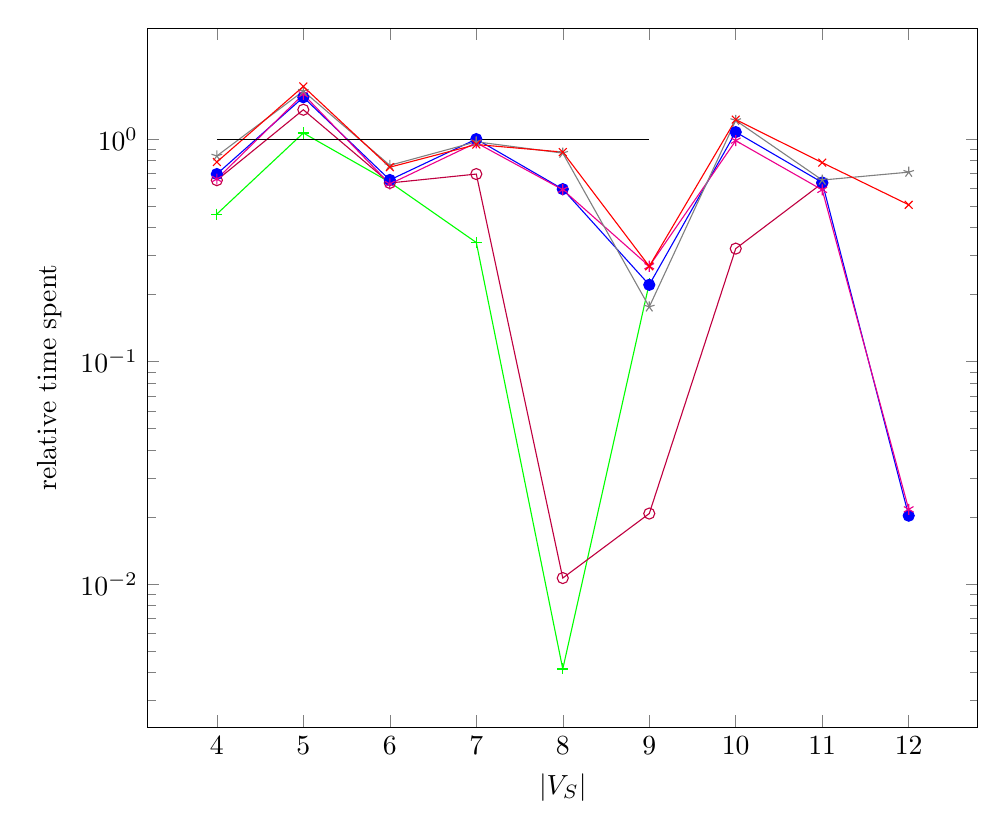
\begin{tikzpicture}
    \begin{axis}[
        xlabel=$|V_S|$,
        ylabel=relative time spent,
        ymode=log,
        legend style={at={(0.9,0.1)},anchor=south east},
        width=\textwidth,
		y tick label style={/pgf/number format/sci},
    ]

\addplot[
        mark=+,
        green,
    ] plot coordinates {
        (4,0.4603454215293834)
        (5,1.0650216337194074)
        (6,0.6402609902641055)
        (7,0.3429545951232229)
        (8,0.004156976828625529)
        (9,0.22489814118245785)
};
 %   \addlegendentry{CP}
    
    \addplot[
        mark=o,
        purple,
    ] plot coordinates {
        (4,0.6536194606761304)
        (5,1.3546625727069868)
        (6,0.6349737425008939)
        (7,0.6963677891889153)
        (8,0.010649285020911963)
        (9,0.02075639387474258)
        (10,0.3219692946843138)
        (11,0.6331864854788115)
};
 %   \addlegendentry{GDFS O IP}

\addplot[
        mark=*,
        blue,
    ] plot coordinates {
        (4,0.6964763815520504)
        (5,1.5418767352722276)
        (6,0.655132639298351)
        (7,0.9999288333397025)
        (8,0.5958121258705841)
        (9,0.22131003316388181)
        (10,1.0751746486592535)
        (11,0.6382538165641153)
        (12,0.02029968985193284)
};
  %  \addlegendentry{K-Path}
    
    
    \addplot[
        mark=asterisk,
        magenta,
    ] plot coordinates {
        (4,0.6613792478641376)
        (5,1.5903154443877043)
        (6,0.6283278818175081)
        (7,0.9629244885375634)
        (8,0.5921232096268492)
        (9,0.2682914762370498)
        (10,0.9835719984313271)
        (11,0.5912237044773625)
        (12,0.02168235616079701)
};
  %  \addlegendentry{GDFS A IP}
    
    
    \addplot[
        mark=star,
        gray,
    ] plot coordinates {
        (4,0.8400238494760311)
        (5,1.6432913297339495)
        (6,0.7623783834679656)
        (7,0.9724418464068187)
        (8,0.8649452249859358)
        (9,0.17617155505832582)
        (10,1.212740370430325)
        (11,0.6545125286561274)
        (12,0.7102484891877338)
};
 %   \addlegendentry{GDFS C}
    
    \addplot[
        mark=x,
        red,
    ] plot coordinates {
        (4,0.7890817980923504)
        (5,1.7236983707312352)
        (6,0.7476536478460998)
        (7,0.9454835701186506)
        (8,0.8743040069418077)
        (9,0.2682189465805335)
        (10,1.2231897365346933)
        (11,0.7838936485791846)
        (12,0.5066592201432429)
};
%    \addlegendentry{DFS}

\addplot [mark=none, black] plot coordinates {
        (4,1) (9, 1)};
%\addlegendentry{No contraction}


	
    \end{axis}
    \end{tikzpicture}

\caption{$|V_T|=3|V_S|$}
\end{subfigure}\\[1ex]
\begin{subfigure}{0.5\linewidth}
\centering

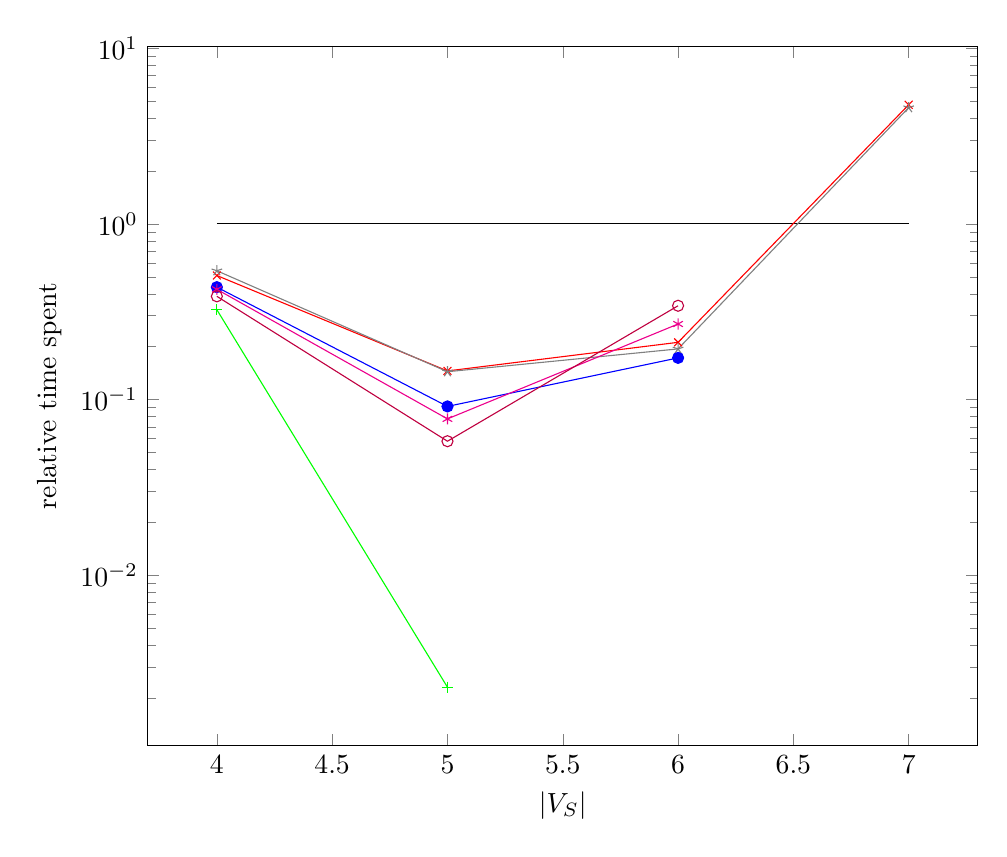
\begin{tikzpicture}
    \begin{axis}[
        xlabel=$|V_S|$,
        ylabel=relative time spent,
        ymode=log,
        legend style={at={(0.9,0.1)},anchor=south east},
        width=\textwidth,
		y tick label style={/pgf/number format/sci},
    ]


\addplot [mark=none, black] plot coordinates {
        (4,1) (7, 1)};
%\addlegendentry{No contraction}
\addplot[
        mark=+,
        green,
    ] plot coordinates {
        (4,0.3247986778213492)
        (5,0.0023085173636887735)
};
%    \addlegendentry{CP}


\addplot[
        mark=x,
        red,
    ] plot coordinates {
        (4,0.5083088516623958)
        (5,0.14560631066960938)
        (6,0.21180693936992814)
        (7,4.763971312568752)
};
 %   \addlegendentry{DFS}


\addplot[
        mark=star,
        gray,
    ] plot coordinates {
        (4,0.5412364762939754)
        (5,0.14410181776854825)
        (6,0.19432561438404647)
        (7,4.587173792533694)
};
%    \addlegendentry{GDFS C}


\addplot[
        mark=*,
        blue,
    ] plot coordinates {
        (4,0.43647426849988535)
        (5,0.09146773493441722)
        (6,0.17275569282732595)
};
 %   \addlegendentry{K-Path}


\addplot[
        mark=asterisk,
        magenta,
    ] plot coordinates {
        (4,0.4241962520645475)
        (5,0.07767539614505417)
        (6,0.26930850582566696)
};
 %   \addlegendentry{GDFS A IP}


\addplot[
        mark=o,
        purple,
    ] plot coordinates {
        (4,0.38706533483340066)
        (5,0.05797333316929685)
        (6,0.34203860563242006)
};
%    \addlegendentry{GDFS O IP}

	
	
    \end{axis}
    \end{tikzpicture}

\caption{$|V_T|=5|V_S|$}
\end{subfigure}
\begin{subfigure} {0.5\linewidth}
\centering

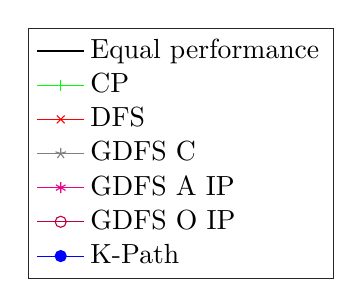
\begin{tikzpicture} 
    \begin{axis}[%
    hide axis,
    xmin=10,
    xmax=50,
    ymin=0,
    ymax=0.4,
    legend style={draw=white!15!black,legend cell align=left}
    ]
	\addlegendimage{black}
    \addlegendentry{Equal performance}; 
     
    \addlegendimage{green, mark=+}
    \addlegendentry{CP};
    
    \addlegendimage{red, mark=x}
    \addlegendentry{DFS};
    
    \addlegendimage{gray, mark=star}
    \addlegendentry{GDFS C};
    
    \addlegendimage{magenta, mark=asterisk}
    \addlegendentry{GDFS A IP};
    
    \addlegendimage{purple, mark=o}
    \addlegendentry{GDFS O IP};
    
    \addlegendimage{blue, mark=*}
    \addlegendentry{K-Path};
    
    \end{axis}
\end{tikzpicture}

\end{subfigure}

\caption{Performance of our algorithm with the degree-based target graph vertex order relative to the performance of the algorithm with a random target graph vertex order. We avoid unnecessarily long paths, do not perform contraction and use no pruning. Data points above the black reference line denote the degree-based ordering introduces more delay, and data points below the reference line denote that it saves time. Note the logarithmic y-axis.}	
\label{fig:greatestDegreeVersusRandom}
\end{figure}
